\documentclass[convert={density=600,size=672x480,outext=.png}]{standalone}
\usepackage{tikz}
\usetikzlibrary{calc, shapes, positioning, decorations.text, arrows.meta,
                trees,positioning,arrows,chains,shapes.geometric,automata,%
                decorations.pathreplacing,decorations.pathmorphing,shapes,%
                matrix,shapes.symbols,plotmarks,decorations.markings,shadows}
\usepackage{tikzscale}
\usepackage{pgfplots}

\definecolor{mybluetikz}{RGB}{86,180,233}
\definecolor{myredtikz}{RGB}{213,94,0}
\definecolor{mygreen}{RGB}{124,174,0}

\definecolor[named]{myblue}{RGB}{0,102,204}
\definecolor[named]{myred}{RGB}{174,49,54}

%%%%%%%%%%%%%%%%%%%%%%%%%%%%%%%%%%%%%%%%%%%%%%%%%
%
% Some definitions for TikZ graphics
%
%%%%%%%%%%%%%%%%%%%%%%%%%%%%%%%%%%%%%%%%%%%%%%%%%

\tikzset{
  root/.style = {rectangle,rounded corners, text width=7em, text centered, inner sep=2mm,
                 align = center, top color=white,
                 bottom color=blue!50!black!20, draw=blue!40!black!60, very thick},
  goodnode/.style = {rectangle, rounded corners, text width = 7em, text centered, inner sep = 2mm,
                     draw = mygreen!60,
                     top color = white, bottom color = mygreen!40, very thick},
  badnode/.style = {rectangle, rounded corners,text width = 7em, text centered, inner sep = 2mm,
                    draw = myredtikz!60,
                    top color = white, bottom color = myredtikz!40, very thick},
  nonode/.style = {rectangle, rounded corners, text width = 7em, text centered, inner sep = 2mm,
                   draw = mybluetikz!60,
                   top color = white, bottom color = mybluetikz!40, very thick}
}

\pgfplotsset{compat = 1.12,
     cmhplot/.style={color=mybluetikz,mark=none,line width=3pt,-},
     cmhplotouter/.style={color=mybluetikz!70,mark=none,line width=3pt,-},
     cmhplotobs/.style={color=mybluetikz,mark=none,line width=2pt,-},
     cmhplotbuys/.style={color=mygreen!40,mark=none,line width=1.5pt,-},
     cmhplotsells/.style={color=myredtikz!40,mark=none,line width=1.5pt,-},
     soldot/.style={color=myredtikz,only marks,mark=*, mark size = 3.5},
     holdot/.style={color=myredtikz,fill=white,only marks,mark=*, mark size = 3.5},
     soldotouter/.style={color=myredtikz!70,only marks,mark=*, mark size = 3.5},
     holdotouter/.style={color=myredtikz!70,fill=white,only marks,mark=*, mark size = 3.5},
     soldotbuys/.style={color=mygreen!40,only marks,mark=*, mark size = 2},
     holdotbuys/.style={color=mygreen!40,fill=white,only marks,mark=*, mark size = 2},
     holdotbuysreset/.style={color=mygreen!40,fill=white,only marks,mark=square*, mark size = 3},
     soldotsells/.style={color=myredtikz!40,only marks,mark=*, mark size = 2},
     holdotsells/.style={color=myredtikz!40,fill=white,only marks,mark=*, mark size = 2},
     holdotsellsreset/.style={color=myredtikz!40,fill=white,only marks,mark=square*, mark size = 3},
     soldotobs/.style={color=mybluetikz,only marks,mark=*, mark size = 2.5},
     holdotobs/.style={color=mybluetikz,fill=white,only marks,mark=*, mark size = 2.5},
}
\begin{document}
\tikzset{
  root/.style = {rectangle,rounded corners, text width = 6em, text centered, inner sep=2mm,
                 align = center, top color=white,
                 bottom color=blue!50!black!20, draw=blue!40!black!60, very thick},
  goodnode/.style = {rectangle, rounded corners, text width = 7em, text centered, inner sep = 2mm,
                     draw = mygreen!60,
                     top color = white, bottom color = mygreen!40, very thick},
  badnode/.style = {rectangle, rounded corners, text width = 7em, text centered, inner sep = 2mm,
                    draw = myredtikz!60,
                    top color = white, bottom color = myredtikz!40, very thick},
  nonode/.style = {rectangle, rounded corners, text width = 6em, text centered, inner sep = 2mm,
                   draw = mybluetikz!60,
                   top color = white, bottom color = mybluetikz!40, very thick}
}

\pgfplotsset{compat = 1.12}

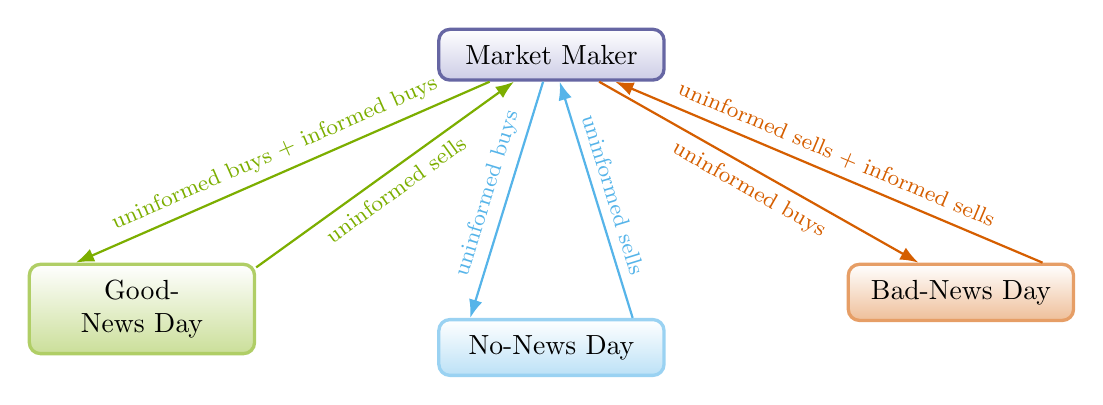
\begin{tikzpicture}[auto]
  \node [root] (MM) {Market Maker};
  \node [nonode, below =3cm of MM] (no) {No-News Day};
  \node [goodnode, below left =3.25cm of MM] (good) {Good-News Day};
  \node [badnode, below right =3.25cm of MM] (bad) {Bad-News Day};

  \path [mygreen, -Latex, thick]
        (MM) edge node[sloped, anchor = center, above] {\footnotesize uninformed buys + informed buys} (good.145)
        (good.20) edge node[sloped, anchor = center, below] {\footnotesize uninformed sells} (MM);

  \path [mybluetikz, -Latex, thick]
        (MM) edge node[sloped, anchor = center, above] {\footnotesize uninformed buys} (no.160)
        (no.20) edge node[sloped, anchor = center, above] {\footnotesize uninformed sells} (MM);

  \path [myredtikz, -Latex, thick]
        (MM) edge node[sloped, anchor = center, below] {\footnotesize uninformed buys} (bad.145)
        (bad.20) edge node[sloped, anchor = center, above] {\footnotesize uninformed sells + informed sells} (MM);
\end{tikzpicture}
\end{document}